\begin{frame}
  % \frametitle{激光的似然域模型---简介}
  \frametitle{激光的似然域模型}
  \begin{itemize}
    \item 不必计算相对于任何有意义的传感器物理生成模型的条件概率,计算更高效。
    \item 这种方法在实践中运行效果良好,即使在混乱的空间,得到的后验也更加光滑。
  \end{itemize}
\end{frame}

\begin{frame}
  % \frametitle{激光的似然域模型---算法步骤1}
  \frametitle{激光的似然域模型}
  \begin{itemize}
    \item 首先将传感器扫描的终点$z_t$映射到地图的全局坐标空间。
    \item 机器人在t时刻的位姿为$x_t = (x,y, \theta)^T$,
          传感器的安装位置相对于机器人的中心坐标$(x_{k, sens}, y_{k, sens})^T$,
          激光光束相对于机器人的朝向的角度为$\theta_{k, sens}$,
          激光光束测量到的距离值为$z_t^k$ 。
          激光扫描到的点投影到地图的全局坐标系坐标为$(x_{z_t^k}, y_{z_t^k})^T$,如式\ref{eq:siranquan}所示。
  \end{itemize}

  \begin{eqnarray}
    \begin{pmatrix}
      x_{z_t^k} \\ y_{z_t^k}
    \end{pmatrix}
    = 
    \begin{pmatrix}
      x \\ y
    \end{pmatrix}
    +
    \begin{pmatrix}
      \cos\theta \quad -\sin\theta \\
      \sin \theta \qquad \cos\theta
    \end{pmatrix}
    \begin{pmatrix}
      x_{k, sens} \\ y_{k, sens}
    \end{pmatrix}
    +
    z_t^k
    \begin{pmatrix}
      \cos(\theta + \theta_{k, snes}) \\ \sin(\theta + \theta_{k, sens})
    \end{pmatrix}
    \label{eq:siranquan}
  \end{eqnarray}
\end{frame}

\begin{frame}
  % \frametitle{激光的似然域模型---算法步骤2}
  \frametitle{激光的似然域模型}

  \begin{itemize}
    \item 似然域模型假设存在三种类型噪声和不确定性。即测量噪声$p_{hit}$、测量失败$p_{max}$、无法解释的随机测量$p_{rand}$。

  \end{itemize}

  \begin{enumerate}
    \item 测量噪声$p_{hit}$。由测量过程引起的噪声使用高斯进行建模。用$dist$表示测量坐标$(x_{z_t^k}, z_{z_t^k})$与地图$m$上最近物体之间的欧式距离。
          因此传感器测量概率可以用均值为0的高斯函数表示: $$p_{hit}(z_k^t|x_t, m) = \mathrm{\epsilon}_{\sigma_{hit}}(dist)$$
  \end{enumerate}

  \begin{figure}[htbp]
  %   \centering
  %   \subfigure[酒店服务送机器人]{
  %   \begin{minipage}[t]{0.45\linewidth}
  %   \centering
    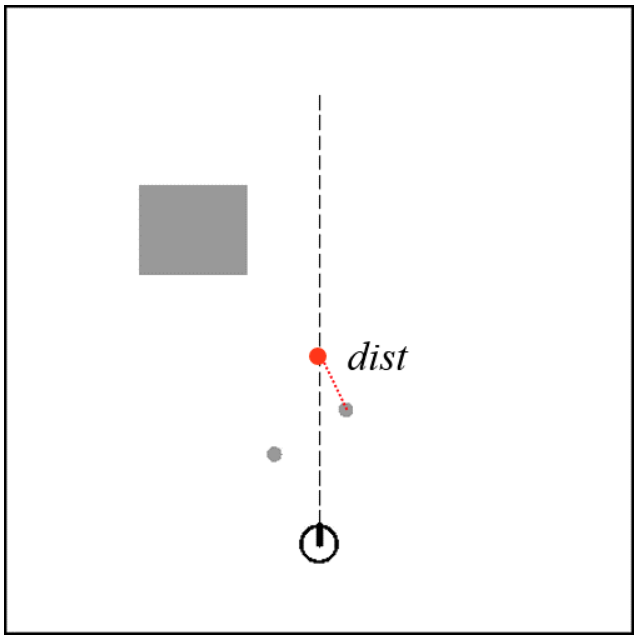
\includegraphics[trim=0mm 0mm 0mm 0mm,clip,height=2.5cm]{amcl/siranyu1}
  %   \label{fig:1gaoxian}
  %   \end{minipage}%
  %   }%
  %   \subfigure[外墙面检查机器人]{
  %   \begin{minipage}[t]{0.45\linewidth}
  %   \centering
    % \includegraphics[trim=0mm 0mm 0mm 0mm,clip,width=5.5cm,height=4.5cm]{1qiangmian}
    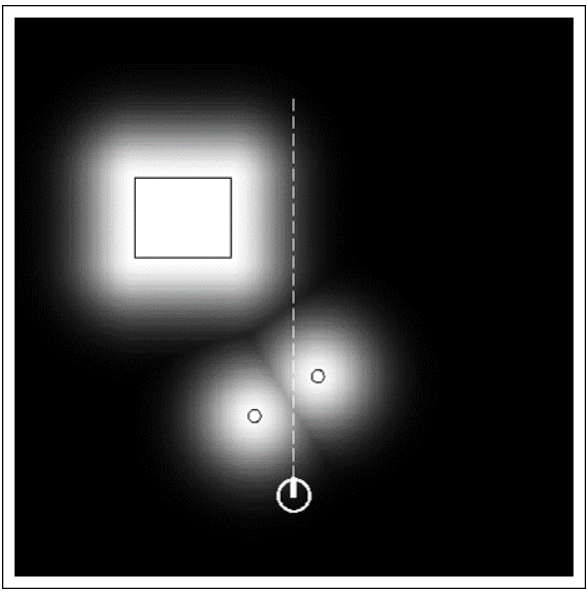
\includegraphics[trim=0mm 0mm 0mm 0mm,clip,height=2.5cm]{amcl/siranyu2}

  %   \label{fig:1qiangmian}
  %   \end{minipage}%
  %   }%
  \end{figure}


\end{frame}

\begin{frame}
  % \frametitle{激光的似然域模型---算法步骤2}
  \frametitle{激光的似然域模型}

  \begin{enumerate}
    \setcounter{enumi}{1}
    \item 测量失败。假定最大距离读数具有非常大的似然值,可用点群分布$p_{max}$进行建模。
    \item 无法解释的随机测量。用一个均匀分布$p_{rand}$描述。
  \end{enumerate}

  \begin{itemize}
    \item 最后,已知$t$时刻位姿$x_t$和地图$m$的情况下,则观测到$z_t^k$的概率$p(z_t^k | x_t, m)$:
          $$p(z_t^k|x_t, m) = z_{hit} \cdot p_{hit} + z_{rand} \cdot p_{rand} + z_{max} \cdot p_{max}$$
          其中$z_{hit}$,$z_{rand}$,$z_{max}$为权重。
  \end{itemize}
  % 最后,已知$t$时刻位姿$x_t$和地图$m$的情况下,则观测到$z_t^k$的概率$p(z_t^k | x_t, m)$:
  %         $$p(z_t^k|x_t, m) = z_{hit} \cdot p{hit} + z_{rand} \cdot p{rand} + z_{max} \cdot p{max}$$
  %         其中$z_{hit}$,$z_{rand}$,$z_{max}$为权重。
\end{frame}

\begin{frame}[fragile]
  % \frametitle{激光的似然域模型---算法}
  \frametitle{激光的似然域模型}

  \begin{columns}
    \column{0.05\textwidth}
    \column{0.9\textwidth}
    \begin{block}

        \begin{algorithmic}[1]
          \State Algorithm likelihood\_field\_model$(z_t, x_t, m)$:
          \State $q = 1$
          \State for all $k$ do
          \State \quad if $z_t^k \neq z_{max}$
          \State \qquad $x_{z_t^k} = x + x_{k, sens} \cos\theta - y_{k, sens} \sin\theta + z_t^k \cos(\theta + \theta_{k, sens})$
          \State \qquad $y_{z_t^k} = y+y_{k, sens}\cos\theta+x_{k, sens}\sin\theta+z_t^k \sin(\theta + \theta_{k, sens})$
          \State \qquad $dist = \substack{\text{min}\\x^\prime, y^\prime} \left\{ \sqrt{(x_{z_t^k}-x^\prime)^2 + (y_{z_t^k} - y^\prime)^2} | \left \langle x^\prime, y^\prime \right \rangle\text{occupied in m} \right\}$
          \State \qquad $q = q \cdot (z_{hit} \cdot prob(dist, \sigma_{hit}) + \frac{z_{random}}{z_{max}})$
          \State return $q$
        \end{algorithmic}
    \end{block}
    \column{0.05\textwidth}
  \end{columns}
\end{frame}

\begin{frame}[fragile]
  \frametitle{代码分析}
  \begin{lstlisting}[frame=shadowbox]  
    //激光雷达位姿变换到全局坐标系下
    pf_vector_t  pf_vector_coord_add(pf_vector_t a, pf_vector_t b) 
    {
      pf_vector_t c;
      c.v[0] = b.v[0] + a.v[0] * cos(b.v[2]) - a.v[1] * sin(b.v[2]);
      c.v[1] = b.v[1] + a.v[0] * sin(b.v[2]) + a.v[1] * cos(b.v[2]);
      c.v[2] = b.v[2] + a.v[2];
      c.v[2] = atan2(sin(c.v[2]), cos(c.v[2]));
      return c;
    }
    ......
    //激光雷达的每个光束末端位置变换到全局坐标系下
    hit.v[0] = pose.v[0] + obs_range * cos(pose.v[2] + obs_bearing); 
    hit.v[1] = pose.v[1] + obs_range * sin(pose.v[2] + obs_bearing);
  \end{lstlisting}
\end{frame}

\begin{frame}[fragile]
  \frametitle{代码分析}
  \begin{lstlisting}
    //计算似然域
    void map_update_cspace(map_t *map, double max_occ_dist)
    {
      unsigned char* marked;
      std::priority_queue<CellData> pq;

      marked = new unsigned char[map->size_x * map->size_y];
      memset(marked, 0, sizeof(unsigned char) * map->size_x * map->size_y);
      map->max_occ_dist = max_occ_dist;

      CachedDistanceMap* cdm = get_distance_map(map->scale, map->max_occ_dist);

      CellData cell;
      cell.map_ = map;
  \end{lstlisting}
\end{frame}

\begin{frame}[fragile]
  \frametitle{代码分析}
  \begin{lstlisting}
      //将地图中表示障碍物栅格push到优先队列中
      for(int i=0; i<map->size_x; i++) {
        cell.src_i_ = cell.i_ = i;
        for(int j=0; j<map->size_y; j++) {
          if(map->cells[MAP_INDEX(map, i, j)].occ_state == +1) {
            map->cells[MAP_INDEX(map, i, j)].occ_dist = 0.0;
            cell.src_j_ = cell.j_ = j;
            marked[MAP_INDEX(map, i, j)] = 1;
            pq.push(cell);
          }
          else 
            map->cells[MAP_INDEX(map, i, j)].occ_dist = max_occ_dist;
        }
      }
  \end{lstlisting}
\end{frame}

\begin{frame}[fragile]
  \frametitle{代码分析}
  \begin{lstlisting}
      //传播算法计算似然域
      while(!pq.empty()) {
        CellData current_cell = pq.top();
        if(current_cell.i_ > 0)
          enqueue(map, current_cell.i_-1, current_cell.j_, current_cell.src_i_, current_cell.src_j_, pq, cdm, marked);
        if((int)current_cell.i_ < map->size_x - 1)
          enqueue(map, current_cell.i_+1, current_cell.j_, current_cell.src_i_, current_cell.src_j_, pq, cdm, marked);
        ......
        pq.pop();
      }
      delete[] marked;
    }
  \end{lstlisting}
\end{frame}

\begin{frame}[fragile]
  \frametitle{代码分析}
  \begin{lstlisting}
    void enqueue(map_t* map, int i, int j, int src_i, int src_j, 
        std::priority_queue<CellData>& pq, CachedDistanceMap* cmd, unsigned char* marked)
    {
      if(marked[MAP_INDEX(map, i, j)]) return;
      int di = abs(i - src_i);
      int dj = abs(j - src_j);
      double distance = cmd->distances_[di][dj];
      if(distance > cmd->cell_radius_) return;
      map->cells[MAP_INDEX(map, i, j)].occ_dist = distance * map->scale;

      CellData cell; cell.map_ = map;
      cell.i_ = i; cell.j_ = j; cell.src_i_ = src_i; cell.src_j_ = src_j;
      pq.push(cell);
      marked[MAP_INDEX(map, i, j)] = 1;
    }
  \end{lstlisting}
\end{frame}

\begin{frame}
  \frametitle{激光的似然域模型的优缺点}
  \begin{itemize}
    \item 优点
    \begin{enumerate}
      \item 光滑性较好,机器人位姿$x_t$的微小改变仅对分布结果$p(z_t^k|x_t,m)$有很小的影响。
      \item 寻找最近障碍物是最耗时的,不过可以通过预计算似然域,搜索时直接查表即可。总的来说该算法较为简单,计算速度也相对较快。
    \end{enumerate}
    \item 缺点
    \begin{enumerate}
      \item 它不能对人或可能引起短读数的其他动态障碍物清晰地建立模型。
      \item 在传感器数据计算障碍点时没有考虑到传感器不能“穿墙”,也就是不能确定到一个点的路径是否被地图上的障碍物所拦截。
      \item 似然域模型没有考虑地图的不确定性,它不能处理地图上不确定或不明确的未探索区域。
    \end{enumerate}
  \end{itemize}
\end{frame}